% this file is called up by thesis.tex
% content in this file will be fed into the main document
% change according to folder and file names
\ifpdf
    \graphicspath{{3/figures/PNG/}{3/figures/PDF/}{3/figures/}}
\else
    \graphicspath{{3/figures/EPS/}{3/figures/}}
\fi

%: ----------------------- name of chapter  -------------------------
\chapter{Description of the proposed two-step algorithm} % top level followed by section, subsection
\label{OurMethod}
\section{Derivation of the algorithm}
In this section, we describe in detail the way our proposed algorithm was conceived and derived. 
\subsection{Drawbacks of the existing online algorithms}
\begin{figure}[t]
		\centering
		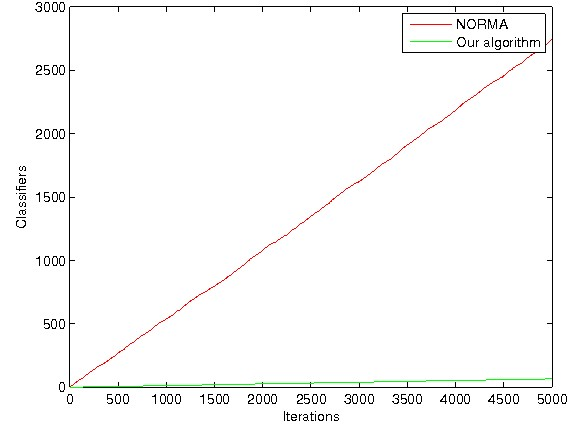
\includegraphics[width=0.8\textwidth]{NORMAOursGrowth}
		\caption[Number of classifiers evaluated per iteration, NORMA and our algorithm]{Number of classifiers evaluated per iteration, signifying complexity growth over training iterations, NORMA and our algorithm at $r=75$}
		\label{NORMAOurs}
	\end{figure}
\begin{figure*}[t]
    \centering
\begin{subfigure}[b]{.45\linewidth}
       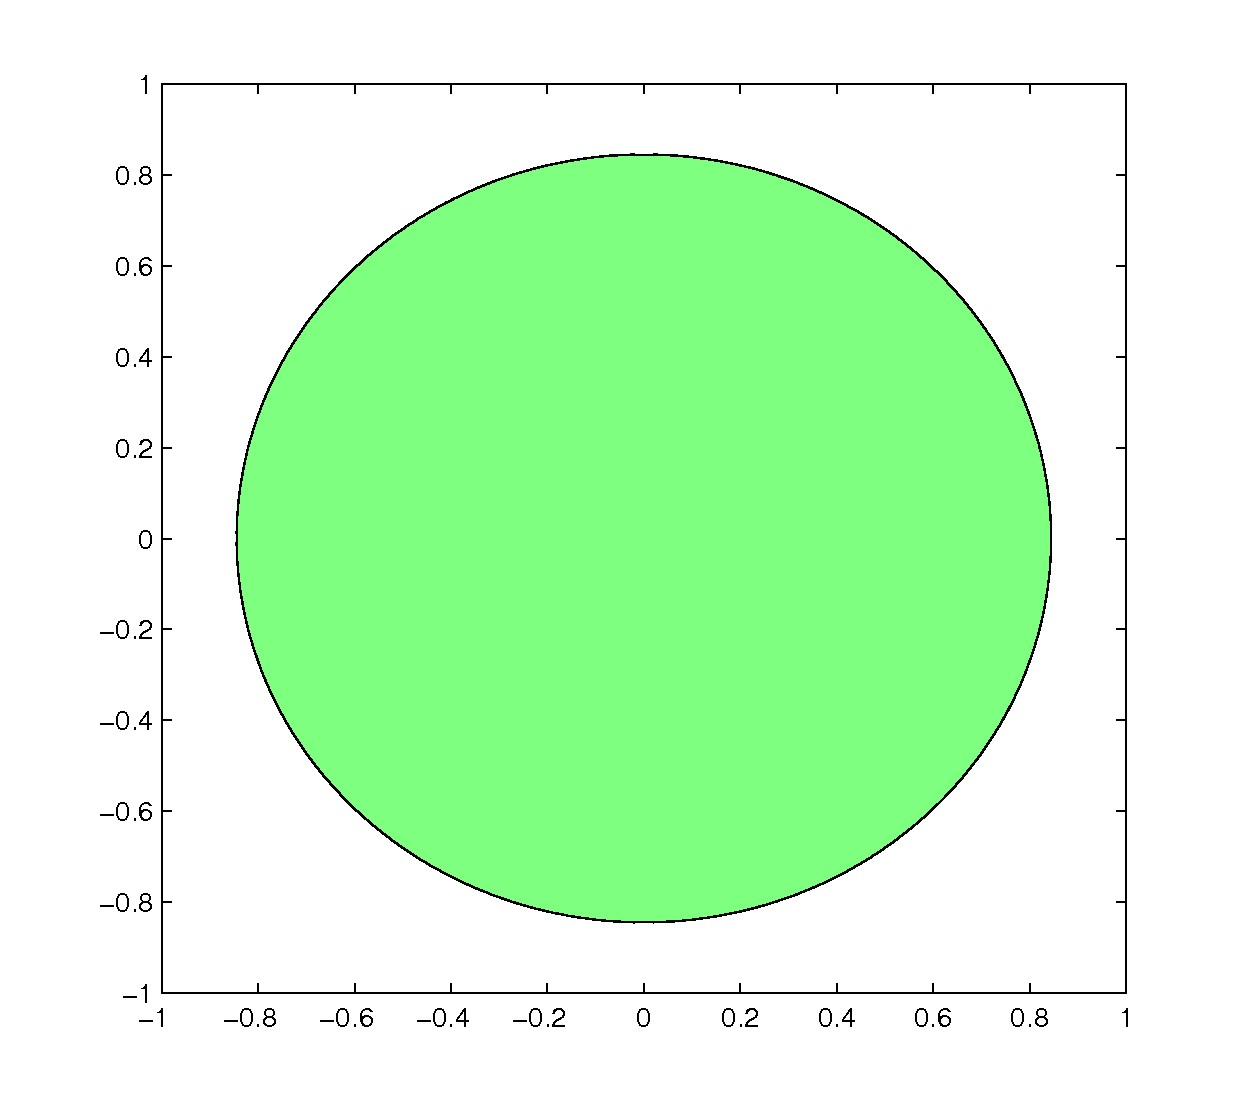
\includegraphics[width=0.9\linewidth]{Target}
\label{apTarget}
        \caption{Target separation area, generated by a single RBF function}
      \end{subfigure}%
\hspace{.01\linewidth}
\begin{subfigure}[b]{.45\linewidth}
	 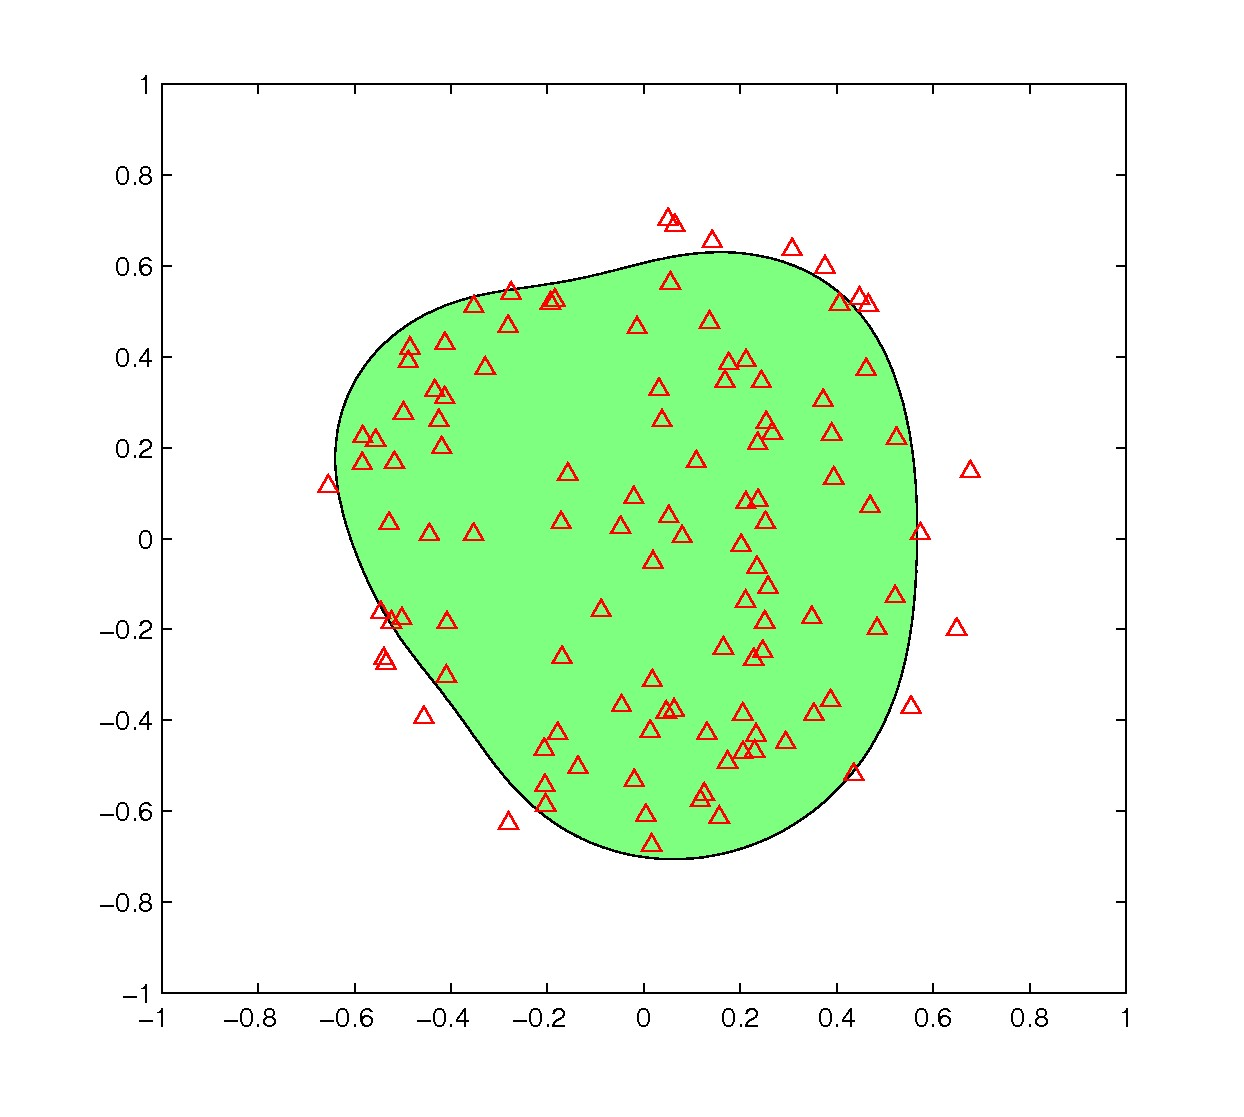
\includegraphics[width=0.9\linewidth]{resultApp}
       \label{apResult}
      \caption{Result of SVM training approximates target area with a large number of kernels}
  
	 \end{subfigure}%

    \caption{Approximation of the target area by the RBF kernel}
    \label{approx}
\end{figure*}
The method described in chap. \ref{Chap2} represent, in a certain way, two extremes of a spectrum. On one hand, the SVM training algorithms like Pegasos and NORMA may be used for either linear classification, which is fast and has low memory requirements, but has the drawback of being of limited utility, since the majority of data distributions in the natural datasets is nonlinear, or nonlinear kernel-based classification, which is imprecise in the case the optimal kernel for the data distribution is unknown, and, even in the optimal case, often exhibits growth of computational complexity by accumulating kernel expansion coefficients, that is roughly proportional to half the the processed data (see \figref{NORMAOurs}). The reason for this growth is partially explained by the fact that the provided data points cannot perfectly describe distribution of data in the transformed feature space, and thus the algorithms has to compensate with the larger number of samples to provide approximation (see \figref{approx}). In this way, the kernel versions of the SVM training algorithms represent algorithms with unlimited complexity growth over time.

On the other hands, online boosting algorithms presented in several sources (for example, see \cite{grabner2008}, \cite{chang}, etc) usually adopt the approach of a fixed complexity opposite to that of the offline boosting by fixing the number of classifiers being added to the model at the beginning of the training, which limits the possibly accuracy. They are also limited by the need to estimate and update a large number of pre-selected classifiers on each iteration, although this problem is somewhat mitigated by the simplicity of the classifiers.

Our goal in this paper is to develop a middle-ground classifier that can provide adjustable levels of complexity growth or decay depending on the needs of the application. For that reason, we took a look at a structure of a single AdaBoost update and have adapted it to the online setting by using SVM training as a method of choosing the next classifier.

\subsection{Similarity of AdaBoost and linear SVM}

We shall start the explanation of our algorithm by noting the similarity between a classifier resulting from a linear SVM training and strong classifier of AdaBoost (this similarity being analyzed in more detail in \cite{Boostsvm}). It is easy to see, that \eqrefr{ClassifierOutput} and\eqrefr{BoostingClassifier} are identical, both being the sign value of a confidence function, which in turn is a linear combination of an input. The main difference is in the fact that in case of boosting the original inputs $\vec{x}_i$ were transformed by a set of classifiers to a kind of binary-valued feature space. However, one cannot assume that this makes boosting completely equivalent to the kernel-based SVM, since the $sign$ function, as well as sigmoid function, the extreme case of which it is does, in fact, not satisfy Mercer condition, this fact proven in \cite{smola2001}. This makes direct application of kernel SVM-related methods unpredictable. However, if we were to treat a vector of weak classifier outputs $h_t(\vec{x})$ as a kind of input vectors to the linear SVM classifier, we could use online SVM adaptation to iteratively change the weights $\beta_i$ in the  \eqrefr{BoostingClassifier}.


\subsection{Adapting AdaBoost to online setting by using modified Pegasos algorithm}

AdaBoost iteration consists, essentially, from the two parts - the selection of the weak classifier $h_t(\vec{x})$ minimizing error in respect to the weights provided by the iteration's strong classifier, and selection of the weight for that classifier. 

In the online setting, however, we do not have the option of evaluating each datapoint for each classifier to determine the optimum, although error values on the unweighted dataset can be estimated simply by adding the error of each consecutive iteration. It is also not possible to reach back and reevaluate data points when the weights of the classifiers placed earlier in the AdaBoost iteration chain change due to the changed accuracy estimate. The solution to this problem employed in \cite{OnlineBoost} is to both fix the number of classifiers and to separate them into unrelated sets called selectors (although the latter requirement is relaxed in the later articles \cite{grabner2009}), resulting in the totality of classifiers in each selector to slowly adapt their accuracy values according to their position in the booster chain.

Our solution, however, is to add a single classifier (linear SVM) at a time and then train it according the the weights provided by the current strong classifier, which is also being trained to better fit the global data distribution. This training can be achieved in the variety of ways, but the similarity between the Adaboost and the SVM described in the previous section has lead us to consider one of the online SVM training algorithm for adjusting the boosting weights. Given the simplicity and the higher convergence rate we have chosen Pegasos as our basis training method. 

The online setting also naturally raises the question of calculating the weight of each incoming data point for training the additional classifier.  To answer this, we consider the weights provided by the AdaBoost algorithm at a given iteration $t$
$$
D_{i,t} = e^{-\beta_1 h_1(x_i) y_i}e^{-\beta_2 h_2(x_i) y_i}\cdots e^{-\beta_t h_t(x_i) y_i}=e^(-y_i F(\vec{x_i}))
$$
That is, the weight for each data point is a constant $e$ to the power of the confidence function of the currently available multiplied by the opposite of a given label, which results in a positive value in case the current version of the strong classifier misclassifies the sample and negative if the available classification if correct. Since in our algorithm the we have constant access to the confidence function of the updated strong classifier, the calculation of the weight is relatively straightforward. Several loss functions can be used, including exponential function as in AdaBoost, or the hinge loss function (\eqrefr{Hingeloss}) common to SVM, with varying results, which will be explored later in more detail. 
\subsection{Linear SVM as weak classifiers}
\begin{figure}[t]
		\centering
		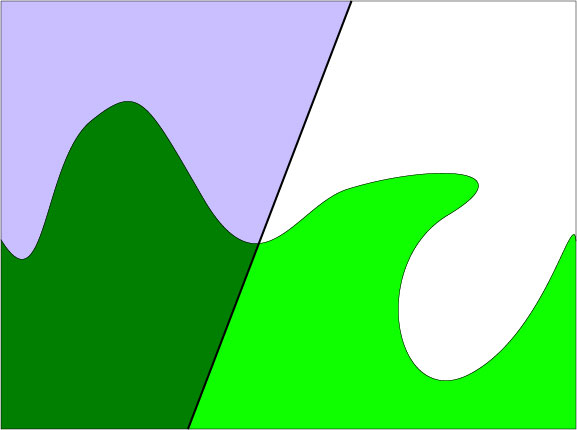
\includegraphics[width=0.6\textwidth]{linearsample2}
		\caption[Example of a random linear classifier]{Example of random linear classifier separating tarhet distribution. It is almost impossible to randomly create a classifier that separates the distribution exacly in half, resulting in error rate of 0.5.}
		\label{linsam}
	\end{figure}
The last step in defining our algorithm is the definition of the weak classifier. In our work, we use a linear SVM for that purpose. Even a random linear classifier would provide an error rate differing from random classification value of $0.5$, in all but extremely rare degenerate cases, which is the only requirement for the weak classifier in AdaBoost (see \figref{linsam} for illustration).

The accuracy of the SVM is then improved by it being trained online by the same Pegasos algorithm as the global classifier with a single difference being an adaptation to the weights provided by the global classifier. Pseudocode and required parameters for the weighted for Pegasos iteration are shown on\figref{PegasosAl}. It should be noted that this is not the only way to incorporate weights into the online update algorithm. For example, \cite{OZ}, as well as \cite{grabner2008} propose using several updates in a row with the number being drawn according to the Poisson distribution. However, we find our adaptation much simpler, and sufficient in terms of accuracy. 
\begin{figure}[t]
		\centering
		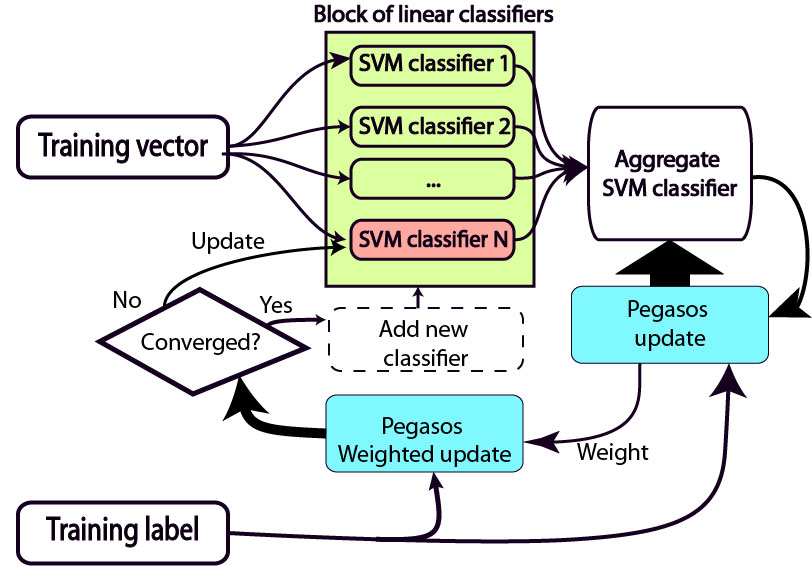
\includegraphics[width=0.8\textwidth]{OurmethodTrain}
		\caption[A diagram of our method]{A diagram of our method}
		\label{schema}
	\end{figure}
\floatstyle{boxed}
\restylefloat{figure}
\begin{figure}[t]

\begin{algorithmic}

\Function {Pegasos}{$\vec{w},\lambda,\vec{x},y,t_w,c$}

$l=\max (0, 1-\vec{w}\cdot\vec{x}y)$

$\sigma=I(l>0)$

$\eta=\frac{1}{\lambda{t}}$

$\vec{w}=(1-\eta\lambda)\vec{w}+{c}\sigma\eta{y}{\vec{x}}$

$\vec{w}=min\left(1,\frac{1}{||\vec{w}||_2\sqrt{\lambda}}\right)\vec{w} $
\EndFunction
\end{algorithmic}
\caption[The Pegasos algorithm with weighted samples]{The Pegasos algorithm with weighted samples. Parameters: $\vec{w}$ - weight vector for the linear SVM, $\lambda$ - regularization parameter, $\vec{x}$ -input training sample, $y$ - training label, $t_w$ - number of current iteration for weak classifier, $c$ - weight parameter 
}
\label{PegasosAl}
\end{figure}
\floatstyle{plain}
\restylefloat{figure}
\section{Description of the resulting algorithm}
\subsection {Algorithm description}
The proposed algorithm  can the be summarized as follows: 
\begin{itemize}
\item It takes 3 parameters, $\lambda$, $\lambda_H$, and parameter $r$ regulating the complexity growth.
\item On each iteration, it takes the following inputs: number of iteration $t$, the number of iterations the weak classifier has been trained $t_w$, $\vec{x}$, $y$, and the outputs of the previous iterations: vectors $\vec{w}_k$, $k=1\cdots K$, $K$ being the number of SVM serving as weak classifiers already incorporated into a strong classifier, and $\vec{\beta}=\beta_1 \cdots\beta_K$ as boosting coefficients for weak classifiers.  On the first iteration, $\vec{w}_1=\vec{0}$, $K=1$, $\beta_1=1$ that is, the classifier being trained is considered incorporated into a strong classifier. 
\item Outputs of weak classifiers are calculated and accumulated into a vector $\vec{h}=h_1\cdots h_K$, $h_k=sign(\vec{w}_k\cdot \vec{x})$ 
\item Confidence function for the resulting global classified is calculated and used to estimate the weight for the training of weak classifier: $F(\vec{h})=\vec{\beta}\cdot \vec{h}$, $c=l(F(\vec{h})$, l defined as a hinge-loss function (\eqrefr{Hingeloss})
\item Weak classifier currently in training (defined by vector $\vec{w}_K$) is updated according to the algorithm illustrated on fig. \ref{PegasosAl}.
\item Vector $\beta$ of the strong classifier is updated using Pegasos algorithm without weight modification, using the calculated confidence value $F$ and regularization parameter $\lambda_H$.
\item Parameters $t$ and $t_w$ are increased: $t=t+1$, $t_w=t_w+1$. 
\item If $t_w>r$, the values of $\vec{w}_K$ are fixed and a new weak classifier is initialized: $K=K+1$, $\vec{w}_K=\vec{0}$,  $\beta_K=0$. Since the classifier is initialized with $0$, it does not start to affect strong classifier $H$ until the next update.
\end{itemize}
This algorithm is illustrated on \figref{schema}

Furthermore, to increase the flexibility of the resulting algorithm, both the weak and the strong classifiers are assumed to incorporate a bias term into an input vector, according to the method described in \cite{rop}, that is, both $\vec{x}$ and $\vec{\beta}$ are assumed to have an additional element equal to $1$. 

From the above definition, it is easy to see that at each iteration our algorithm has a strong classifier ready, same as \cite{OnlineBoost}. The additional parameter $r$ is used to control the complexity and non-linearity of the output, although the experiments have shown that for most non-linear application, the constant value of $r$ about $100$ is sufficient. Higher values of $r$ result in a fewer number of better-trained classifiers combined into a strong classifiers, limiting possible task complexity, while lower result in the weak classifiers  being closer to random and increase complexity without appreciable increase in accuracy for most datasets. 

The result is an algorithm with controllable storage and computational requirements that can be used for online training of strong classifiers on nonlinear data distribution without the use of kernels, and therefore without the need to adjust or fine-tune kernel parameters. Experiments in section \ref{ExperimentsNorma} show that a constant value of parameters works well enough for most complex datasets, proving the simplicity and large applicability range of proposed method. 
\begin{figure*}[t]
    \centering
\begin{subfigure}[b]{.45\linewidth}
       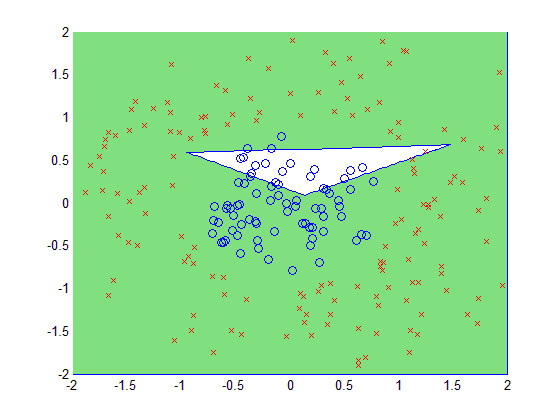
\includegraphics[width=0.9\linewidth]{c1}
\label{Contour1}
        \caption{Separation area generated by our method after first 5 classifiers were added}
      \end{subfigure}%
\hspace{.01\linewidth}
\begin{subfigure}[b]{.45\linewidth}
	 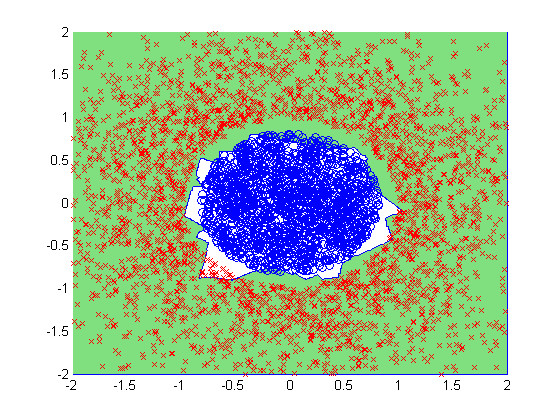
\includegraphics[width=0.9\linewidth]{c2}
       \label{Contour2}
      \caption{Separation area generated by our method after 100 classifiers were added, nearing convergence}
  
	 \end{subfigure}%

\begin{subfigure}[b]{.45\linewidth}
       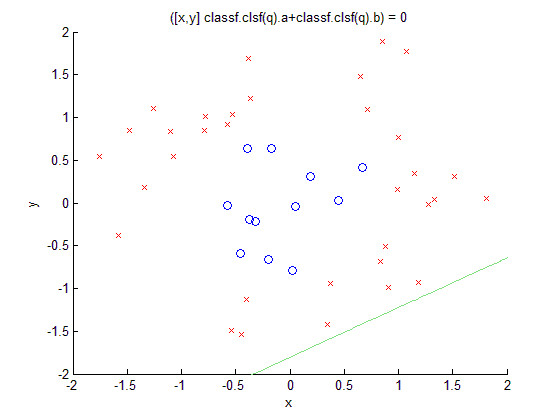
\includegraphics[width=0.9\linewidth]{l1}
\label{lines1}
        \caption{First linear (weak) classifier added by our method}
      \end{subfigure}%
\hspace{.01\linewidth}
\begin{subfigure}[b]{.45\linewidth}
	 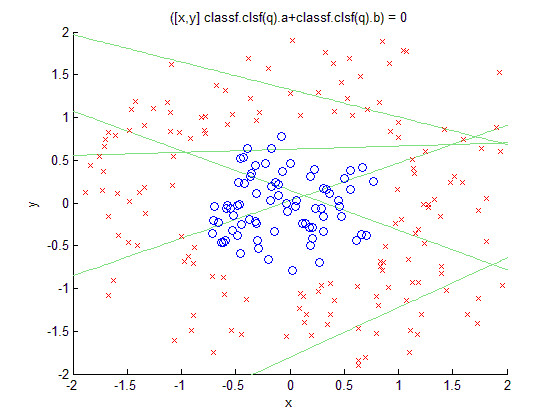
\includegraphics[width=0.9\linewidth]{l2}
       \label{lines2}
      \caption{First 5 classifiers added}
  
	 \end{subfigure}%
    \caption{Example of our method converging to  a target distribution on a sample dataset.}
    \label{convo}
\end{figure*}

\begin{figure}[t]
		\centering
		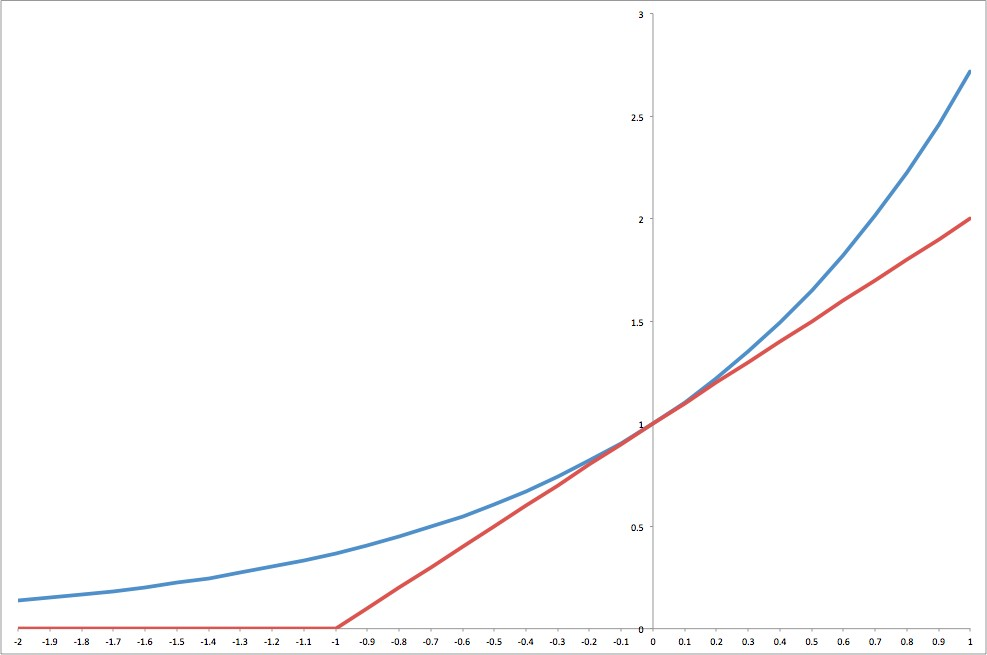
\includegraphics[width=0.7\textwidth]{losses}
		\caption[Loss functions illustrated]{Two loss function popular for use in optimization and SVM training: exponential(blue) and hinge-loss(red) }
		\label{losses}
	\end{figure}
The convergence of our method on a sample 2-dimensional dataset is illustrated on \figref{convo}
\subsection {Possible modifications}
The above algorithm can be modified in several ways to adapt for a specific application requirements or for increased flexibility

{\bf Different loss functions for weak classifier training. }
The function $l$ used to calculate weight for weak classifier training can be changed to, essentially, any monotonically increasing function. Two loss functions popular in optimization are shown on \figref{losses}.  

{\bf Removal of weak classifiers}
While our algorithm allows for accuracy levels comparable or higher to that of kernel-based SVM, with much lower computational complexity, computational and storage costs of our algorithm still grow with input samples. One way to stop this growth is to remove those weak classifiers absolute values of coefficients for which fall below a certain threshold, resulting in eventual replacement of ill-fitting classifiers. This technique also increases the flexibility of the method

{\bf Limiting the global iteration number $t$} Since the learning rate of the algorithm decreases proportionally to iteration number $t$, for applications that deal with constantly changing data distribution it is beneficial to limit the growth of the number $t$, stopping the increase at certain threshold corresponding to the level of flexibility desired. 
 
{\bf Varying number and kind of weak classifiers trained simultaneously}  Since the trainer for strong classifier is unaware of a kind and number of weak classifiers being trained, different features may be added when each new weak classifier is initialized, and several distinct classifiers may be trained at once, especially if the setting favors parallel processing. 
This particular modification  is discussed in more detail in the next section.


\subsection{Comparison to other algorithms}
{\bf Online SVM training methods (NORMA and Pegasos)}
Our methods compares favorably to both NORMA and Pegasos in case of nonlinear data distribution, since they allow for much lower computational and storage requirements. If, however, the parameter $r$ is set to values near $1$, our method is reduced to, essentially, fitting a set of random classifiers to data distribution, with the storage and computational requirement approaching those of kernel methods. However, the estimated computational requirements are still somewhat lower that for most commonly used kernels due to the simplicity of the sign function. 

For the case of linearly separable data, our algorithm is essentially indistinguishable from Pegasos, on which it is based, with additional overhead due to added classifiers.
{\bf Online boosting methods}
It is difficult to compare our method to the online boosting methods due to the difference in methodology. In many ways, our methods are quite opposite. Methods proposed in \cite{OnlineBoost} apply learning updates to the preselected set of classifiers based on random features, while our method updates usually only one classifier per iteration. Also, their algorithm assigns weights to classifiers in a manner similar to AdaBoost, all at the same iteration, while ours adjusts the weights iteratively over time. 


%: ----------------------- paths to graphics ------------------------


%: ----------------------- contents from here ------------------------







% ---------------------------------------------------------------------------
%: ----------------------- end of thesis sub-document ------------------------
% ---------------------------------------------------------------------------

